%Diese Zeile bitte -nicht- aendern.
\documentclass[course=erap] {aspdoc}

%eigene Imports
\usepackage{amsfonts}
\usepackage{pgfplots}
\usepackage{ulem}
\usepackage{amssymb}
\usepackage{mathtools}
\usepackage{graphicx}
\pgfplotsset{compat=1.16}


%%%%%%%%%%%%%%%%%%%%%%%%%%%%%%%%%
%% TODO: Ersetzen Sie in den folgenden Zeilen die entsprechenden -Texte-
%% mit den richtigen Werten.
\newcommand{\theGroup}{233} % Beispiel: 42
\newcommand{\theNumber}{A316} % Beispiel: A123
\author{Ludwig Gröber \and Julian Pins \and Daniel Safyan}
\date{Sommersemester 2023} % Beispiel: Wintersemester 2019/20
%%%%%%%%%%%%%%%%%%%%%%%%%%%%%%%%%

% Diese Zeile bitte -nicht- aendern.
\title{Gruppe \theGroup{} -- Abgabe zu Aufgabe \theNumber}

\begin{document}
    \maketitle


    \section{Einleitung}
    In den Bereichen der Control-Theory und Datenverarbeitung gibt es zahlreiche Anwendungen, in denen die Berechnung bestimmter mathematischer Funktionen von großer Bedeutung ist.~\cite{QUELLE_DANIEL}
    Eine dieser Funktionen ist der \textit{Areasinus Hyperbolicus} ($arsinh(x)$), der unter anderem die Beschreibung nichtlinearer Beziehungen und Modellierung von Sättigungsprozessen ermöglicht.
    Um die Genauigkeit und Effizienz solcher Berechnungen zu garantieren, ist es von entscheidender Bedeutung, die Berechnung des $arsinh(x)$ effizient umzusetzen.
    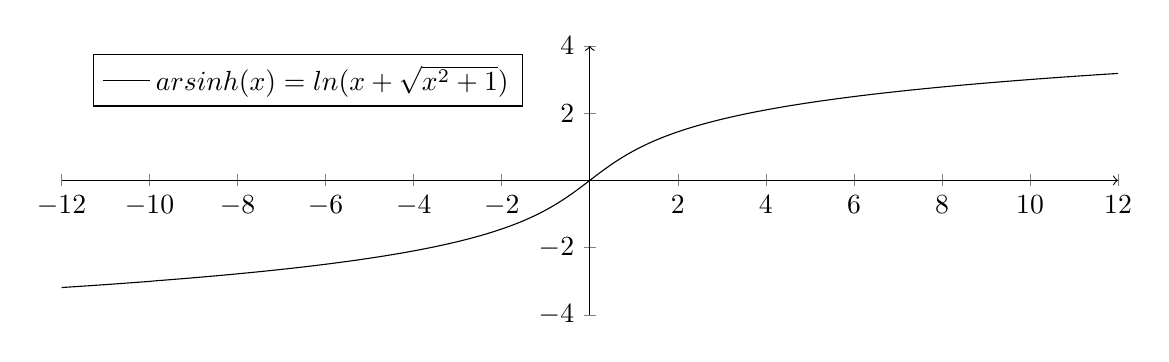
\begin{tikzpicture}
        \begin{axis}
            [
            legend pos = north west,
            width = 15 cm,
            height = 5 cm,
            xmin = -12, xmax = 12,
            ymin = -4, ymax = 4,
            axis lines=middle,
            axis line style={->},
            domain= -20: 20,
            samples = 500
            ]
            \addplot[] {ln(x + sqrt(x*x+1))};
            \legend{$arsinh(x) = ln(x + \sqrt{x^2 + 1})$}

        \end{axis}
    \end{tikzpicture}

    \subsection{Analyse und Spezifikation der Aufgabenstellung}
    Die Aufgabe A316 ist eben diesen $arsinh(x)$ im C17 Standard von C zu approximieren.
    Spezifischer verlangt die Aufgabenstellung explizit zwei Implementierungen, die nur auf einfachen arithmetischen Ausdrücken basiert sowie eine Vergleichsimplementierung, die komplexe Instruktionen benutzen darf.
    Eine dieser Implementierungen soll dabei eine reine Reihe sein, während die andere einen Tabellen-Lookup benutzen soll.

    Für unsere Implementierung wurden folgende Annahmen getroffen:


    Mit der \textbf{"reinen"} \textbf{Reihenentwicklung} ist die Implementierung bezeichnet, welche mit exakt einer Reihendarstellung die Funktionswerte berechnet.
    Fallunterscheidungen nach Intervallen von $x$ dürfen in dieser Implementierung also grundsätzlich nicht gemacht werden.
    Hierbei sollte also eine Reihe gewählt werden, deren Konvergenzbereich am ehesten für ein mögliches Anwendungsgebiet geeignet ist.

    Da die reine Reihenentwicklung nicht für alle Eingabewerte konvergiert wurde eine weitere Implementierung erstellt, die \textbf{mehrere Reihenentwicklungen für verschiedene Intervalle} der Eingabe verwendet.
    Die Anzahl der Fallunterscheidungen soll hierbei minimal gehalten werden, indem möglichst wenige verschiedene Reihenentwicklungen und eine feste Anzahl an berechneten Reihengliedern verwendet werden.

    Für die Implementierung der \textbf{Lookuptabelle} war der Speicherplatz Abwägungskriterium, da für die meisten Anwendungen Speichereffizienz wichtig ist.
    Eine Abwägung zwischen Speicherplatz und Genauigkeit findet sich in Kapitel 2.2.
    Wir haben uns zudem für eine Lookuptabelle mit linearer Interpolation entschieden.

    Als \textbf{Vergleichsimplementierung} verwenden wir die arsinh(x) Funktion der C math Bibiliothek.
    Diese wird in erster Linie für die Bewertung der Genauigkeit herangezogen.
    Es sei an dieser Stelle bereits erwähnt, dass Funktionen der C-Mathematikbibliothek auf Maschinenebene implementiert sind und bestimmte Hardwarefunktionen nutzen können.
    Daher wird diese Implementierung an Performanz kaum zu übertreffen sein.

    Diese vier Implementierungen werden in Kapitel 3 und 4 auf Performanz und Genauigkeit untersucht, verglichen und anhand der Ergebnisse bewertet.


    \section{Lösungsansatz}

    Sowohl für die Implementierung mit einer Reihendarstellung, als auch für die Lookuptabelle haben wir uns die Punktsymmetrie der $arsinh$-Funktion zunutze gemacht: $arsinh(-x) = -arsinh(x)$.
    Die Funktionswerte für negative Eingabewerte werden per Fallunterscheidung mit $-arsinh(|x|)$ berechnet.

    \subsection{ Reihendarstellung}

    \subsubsection{Problematik und Ansätze}

    Bei der Interpolation durch eine reine Reihe der Form $\sum_{k=0}^{\infty} a_k x^k$ bzw. $\sum_{k=0}^{\infty} a_k x^-k$ werden Overflows zum Problem.
    Unabhängig welche Reihe genutzt wird, können die Zwischenergebnisse $x^{\pm k}$ entweder für sehr große Werte oder sehr kleine Werte von $x$ nicht als $double$ dargestellt werden, obwohl das für das Endergebnis nicht gelten muss.
    Deshalb haben Reihendarstellungen stets begrenzten Gültigkeitsbereiche.
    Es wird versucht, eine Reihenentwicklung zu finden, die für einen sinnvollen Konvergenzbereich möglichst genaue Ergebnisse liefert.
    Hierzu haben wir unter anderem die Methode der kleinsten Quadrate verwendet, um geeignet Koeffizienten für Reihenglieder mit positiven oder negativen Potenzen zu finden.
    Die auf diese Weise hergeleitete Reihenentwicklung liefert allerdings für Werte zwischen den verwendeten Datenpunkten sehr ungenaue Ergebnisse, da es sich bei der arsinh-Funktion nicht um ein lineares Modell handelt.
    Wir haben daher stattdessen eine Reihenentwicklung für verschiedene Intervalle hergeleitet, die im Folgenden näher erläutert werden sollen.

    \subsubsection{Umsetzung}

    \[ \operatorname{arsinh}(x) =
    \begin{cases}
        \textit{TaylorArsinh}     & \text{ falls } |x| < 1 \\
        \ln(2x) + error(x)  & \text{ falls } |x| >1 \\
        x     & \text{ falls } x \in \{\pm\inf, \pm Nan\}\\
    \end{cases}\]
    Für bessere Verständlichkeit werden die drei Reihen mit \textit{TaylorArsinh}, \textit{TaylorLn} und \textit{Restreihe} bezeichnet.
    Die Berechnungen werden im Folgenden näher erläutert:

    \subsection{Reihendarstellung für $|x|\leq 1$}
    Für $|x| \leq 1$ wird die Taylor-Reihe des $arsinh(x)$ um den Entwicklungspunkt 0 verwendet:

    \[
        \textit{\textbf{TaylorArsinh}}\coloneqq arsinh(x) = \sum_{k = 0}^{\infty} \frac{(2k-1)!!(-x^2)^k}{(2k)!!(2k + 1)}
        = \sum_{k = 0}^{\infty} \frac{(-1)^k(2k)!x^{2k + 1}}{(2k + 1)(2^k*k!)^2}
    \]

    Durch das Auflösen der Doppelfakultäten entsteht eine leichter implementierbare Formel.

    \subsection{Reihendarstellung für $|x|\geq 1$}
    Die Berechnung für $|x| > 1$ folgt aus folgender Näherung:
    \[
        arsinh(x) = \ln(x + \sqrt{x^2 + 1}) = \ln(2x) + error(x)
    \]
    Der Fehler dieser Näherung kann durch eine dritte Reihe berechnet werden, die vor allem für den Funktionswert von Eingabewerten $|x| < 2^{8}$ notwendig ist:
    \[
        \textit{\textbf{Restreihe}}\coloneqq error(x) =  \sum_{k = 1}^{\infty} \frac{(-1)^{k - 1}(2k)!}{2k(2^k\cdot k!)^2} \cdot \frac{1}{x^{2k}}
    \]

    Für die Berechnung von $\ln(2x)$ wird die Taylor-Reihe des natürlichen Logarithmus um den Entwicklungspunkt 1 verwendet.
    Es ist zu beachten, dass diese Reihe nur im Wertebereich $[0, 2]$ konvergiert.
    \[
        \textbf{\textit{TaylorLn}}\coloneqq\ln(x) = \sum_{k = 1}^{\infty} \frac{(-1)^{k + 1}}{k}(x - 1)^k
    \]
    Aufgrund der begrenzten Gültigkeit der Reihe wird bei der gemischten Implementierung das $double$ Datenformat genutzt, um die Berechnung zu optimieren.
    Durch eine Bitmaske lassen sich effizient Exponent und Mantisse von $x$ ermitteln.
    Mit Exponent und Mantisse lässt sich nun folgende Umformung treffen:
    \begin{gather*}
        x = M\cdot2^E \,\,\, mit \,\,\, M = implizierte Mantisse \,\,\, E = implizierter Exponent\\
        arsinh(x) \approx \ln(2x) = \ln(2) + \ln(x) = \ln(2) + \ln(M\cdot2^E) = \ln(2) + E\cdot\ln(2) + \ln(M)\\
    \end{gather*}
    Da $M\in[1, 2[$ liegt, kann nun \textit{TaylorLn} für die Berechnung von $\ln(M)$ verwendet werden.
    Da die Reihe bereits für wenige Reihenglieder genauere Ergebnisse liefert, je näher der zu berechnende Wert an Eins liegt, haben wir uns dafür entschieden, alle Werte der Mantisse, die über $1.\overline{3}$ liegen, nochmal zu halbieren und stattdessen den Exponenten um 1 zu erhöhen.
    Es gilt $M\in[0.\overline{6}, 1.\overline{3}]$.

    Für eine reine Reihe, die ohne Bitmasken für $x\geq 1$ aussagekräftig ist, benutzen wir die Folgende Umformung:
    \[
        arsinh(x)\approx ln(2x) + error(x) = ln(2) - ln(\frac{1}{x}) + error(x)
    \]
    Dadurch entsteht im Argument des natürlichen Logarithmus wieder ein Wert, wofür die \textbf{TaylorLn}-Reihe gilt.
    Um die reine Reihe zu erhalten, werden die beiden Reihen zu einer vereinigt.
    Durch Ausmultiplizieren der ersten n Reihenglieder lassen sich die Koeffizienten bestimmen und eine herkömmliche Reihe der Form $\sum_{k=0}^{n} a_k x^{-k}$ erstellen.
    Die Koeffizienten der einzelnen Reihenglieder zu berechnen ist laufzeitintensiv, da insbesondere die Berechnung der Fakultät viel Zeit kostet.
    Daher lässt sich die Berechnung optimieren, indem die Koeffizienten aller drei Reihen bereits vor Runtime berechnet werden.
    Durch Anwendung des Horner-Schemas lässt sich nun die Reihe besonders effizient berechnen.

    \subsubsection{Abwägung Genauigkeit und Performanz}
    Die Anzahl an benutzten Reihenglieder, entsteht aus einer Abwägung zwischen Performanz und Genauigkeit.
    Wie viele Reihenglieder berechnet werden müssen, um ein möglichst genaues Ergebnis zu erhalten, hängt von den Eingabewerten ab.
    Da die Reihenglieder aller drei Reihen immer kleiner werden, gilt: Je kleiner das letzte berechnete Reihenglied, desto genauer ist auch das Ergebnis.


    Wir betrachten zunächst \textit{TaylorLn}:
    In der Implementierung liegt der Eingabewert für die Reihe im Intervall $[0.\overline{6}, 1.\overline{3}]$.
    Aus der Formel für das k-te Reihenglied
    \[ \frac{(x - 1)^k}{k}
    \]
    lässt sich errechnen, dass spätestens das 28. Reihenglied dieser Reihe für alle Eingabewerte im gegebenen Intervall $[0.\overline{6}, 1.\overline{3}]$ kleiner als $2^{-50}$ ist.
    Somit würden alle weitere Reihenglieder bei der Addition mit dem Restterm (wegen der Limitierung durch die Mantisse auf 52 bit) nahezu vollständig ausgelöscht werden.
    Wir setzen daher die Anzahl der zu berechnenden Reihenglieder dieser Reihe auf 27.

    Betrachten wir nun \textit{TaylorArsinh}.
    Das k-te Reihenglied hat den Betrag
    \[
        \frac{(2k)!}{(2k + 1)(2^k*k!)^2}\cdot x^{2k+1}
    \]
    Aus dieser Formel lässt sich bereits ablesen, dass ein Reihenglied kleiner ist, je kleiner x ist.
    Die Reihe liefert demnach bereits mit weniger Reihengliedern genauere Ergebnisse, je näher x an 0 liegt.
    Werden versuchsweise bestimmte Werte von x in die Formel eingesetzt, so lässt sich feststellen, dass für x = 0.25 alle Reihenglieder ab dem etwa 13. Glied keinen Einfluss mehr auf das Endergebnis haben.
    Für x = 0.5 müssen 26 Reihenglieder berechnet werden.
    Für x = 0.99 sind bereits etwa 1500 Reihenglieder nötig.

    Für die \textit{Restreihe}, kann eine äquivalente Überlegung getroffen werden, die ebenfalls belegt, dass exponentiell mehr Reihenglieder benötigt werden, je näher x an 1 liegt.

    %TODO: Abbildung

    In der Abbildung ist zu sehen, dass für Eingabewerte nahe an 1 eine unverhältnismäßig hohe Anzahl an Reihengliedern für ein exaktes Ergebnis benötigt werden.
    Aufgrund dieses exponentiellen Wachstums wird die Anzahl der zu berechnenden Reihenglieder für \textit{TaylorArsinh} und \textit{Restreihe} auf 13 festgelegt und damit ein geringer relativer Fehler in den Intervallen $0.25<|x|<4$ in Kauf genommen.
    Diese Abwägung zwischen relativem Fehler und Performanz werden in den folgenden Kapiteln näher untersucht und belegt.

    Es sei an dieser Stelle erwähnt, dass ausgehend von diesen Untersuchungen eine weitere Optimierung umsetzbar wäre, die (beispielsweise mithilfe des Exponenten des Eingabewertes) jeweils die Anzahl der nötigen Reihenglieder bestimmt und dann eben diese (falls die Anzahl kleiner als 13 ist) berechnet.
    Durch diese Optimierung wird zusätzlicher Overhead durch die Berechnung von für das Ergebnis irrelevanten Reihengliedern vermieden.
    Da Fallunterscheidungen ausgeschlossen sind, wurde auf diese Optimierung verzichtet.


    \subsection{Tabellen-Lookup}
    Die Lookuptabelle speichert einige vorberechnete Werte der $arsinh$-Funktion und interpoliert für die verbleibenden Werte linear zwischen den beiden nächstgelegenen Tabellenwerten.
    Bei der Implementierung galt es zunächst zwischen Speicherplatz der Tabelle und Genauigkeit des Ergebnisses abzuwägen.
    Im Rahmen der Ausarbeitung wurde ein Limit von 1 MB für die Lookuptabelle festgelegt.
    Diese Größe ermöglicht das Speichern von rund 40000 Werten.
    Ebenso wurde eine logarithmische Verteilung der Werte festgelegt, da auch die Verteilung aller möglichen Werte im Datentyp $double$ logarithmisch ist.
    Für alle positiven Eingabewerte wurde für jeden möglichen Exponenten $[-1023, +1023]$ eine feste Anzahl an Werten vorberechnet.
    Das gesetzte Speicherlimit beschränkt die Genauigkeit auf 16 Werte pro Exponent.
    Folglich werden 32753 Werte gespeichert.
    Die Folgen dieser Designentscheidung werden im Kapitel Genauigkeit noch näher betrachtet.

    Diese Verteilung ermöglicht zudem ein besonders effizientes Mapping der Eingabewerte auf den zugehörigen Index in der Lookuptabelle durch eine Hashfunktion.
    Durch eine Bitmaske lassen sich Exponent und die ersten 4 Bits der Mantisse ermitteln.
    Diese 15 Bits bilden den Index i des nächstkleineren Wertes in der Lookuptabelle.
    Mit diesem und dem nächsten Tabellenwert gilt $table[i] \leq arsinh(x) < table[i+1]$.
    Daraufhin wird gemäß
    \[
        arsinh(x) \approx \frac{x-x_i}{x_{i+1} - x_i}\cdot (y_{i+1}-y_i) + y_i
    \]
    linear interpoliert.

    \begin{figure}[h]
        \begin{subfigure}
        \centering
        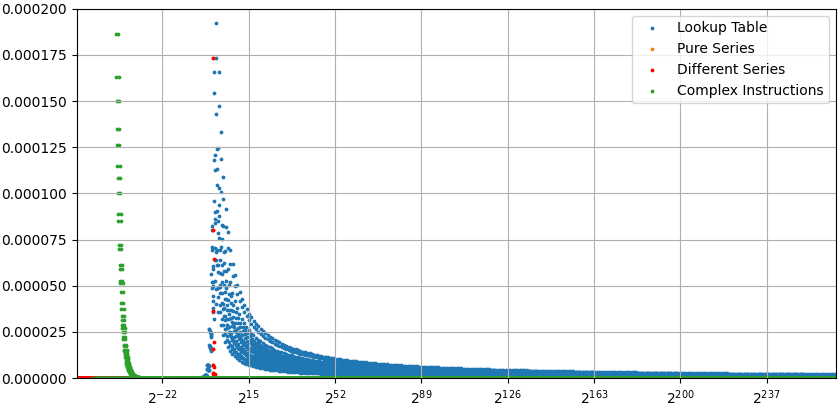
\includegraphics[width = 12cm,height = 8cm]{pdf/Figure3.png}
        \caption{}
        \end{subfigure}
        
        \begin{subfigure}
        \centering
        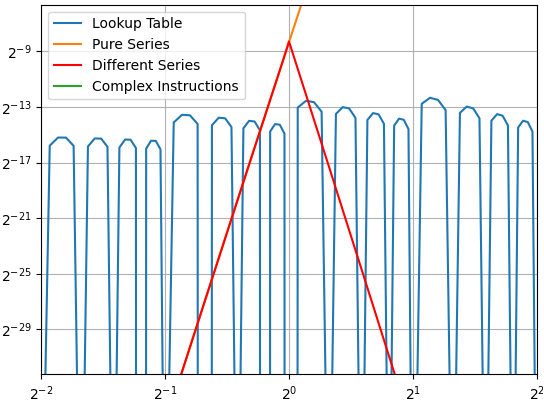
\includegraphics[width = 7cm,height = 6cm]{pdf/Figure1.png}
        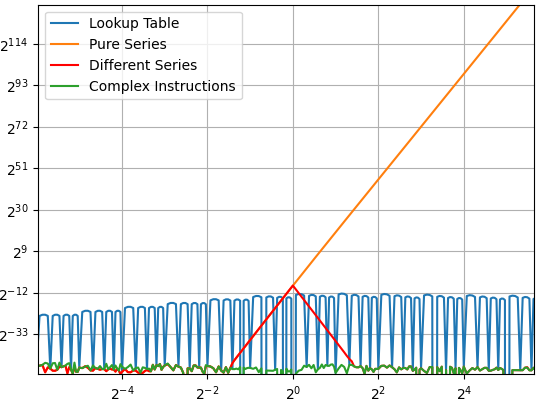
\includegraphics[width = 7cm, height = 6cm]{pdf/Figure2.png}
        \caption{}
        \end{subfigure}
        %\label{fig:enter-label}
    \end{figure}


    \begin{figure}
        \caption{}
    \end{figure}
    Als Maßstab für die Genauigkeit unserer Ergebnisse wird im Folgenden der relative Fehler der Implementierung bezüglich des tatsächlichen mathematischen Funktionswert verwendet. Die folgenden Diagramme wurden erstellt, indem mithilfe einer C-Hilfsmethode für eine große Anzahl an Eingabewerten jeweils die Funktionswerte für alle drei Implementierungen brechnet und in Arrays gespeichert wurden. Anschließend wurden diese Funktionswerte in einem Python-Programm zu den jeweilgen relativen Fehlern ausgewertet und mithilfe der Bibiliothek matplotlib als Graph dargestellt.
    
    \subsection{Reine Reihenentwicklung}
    Wie deutlich in Abb.2.1 erkennbar ist, liefert die Reihenentwicklung außerhalb des Intervalls $0.25<|x|$ nahezu immer den exakten Funktionswert. Es gibt einige Ausnahmen mit einem verschwindend geringen relativen Fehler $\leq2^{-50}$ , welche sich durch floating-point-Rundungsfehler bei der Umrechnung der Polynomkoeffizienten erklären lassen.
    In Abb.2.2 erkennbar, steigt der relative Fehler exponentiell an, je näher der Eingabewert an 1 liegt. Dies lässt sich anhand der Konvergenz der Reihenglieder für verschiedene Eingabewerte erklären. Wie in Kapitel 2.1.1 erläutert, ist das Ergebnis genauer, je kleiner das letzte berechnete Reihenglied ist.
    Wir zeigen zunächst, dass bei 13 Reihengliedern die Grenze für die Entstehung von Ungenauigkeiten bei etwa 0.25 liegt. Hierzu berechnen wir jeweils das letzte Reihenglied für x=0.25:
    \[
    \textit{TaylorArsinh}: \frac{(2\cdot13)!0.25^{2\cdot13 + 1}}{(2\cdot13 + 1)(2^13\cdot13!)^2} \approx 2^{-59}
    \]
    Da des letzte Reihenglied noch unter $2^{-59}$ liegt, hat das Ergebnis noch maximale double Genauigkeit. Für x-Werte näher an 1, wird jedoch das letzte Reihenglied immer größer, wodurch der relative Fehler exponentiell ansteigt. Wie im Graph zu sehen ist, hat die Reihenentwicklung ihren maximalen relativen Fehler von circa $2^{-8} \approx 0.39\%$ am Eingabewert 1.
    Berechnen wir nun das letzte (13.) berechnete Reihenglied für den Eingabewert 1 so erhalten wir:
    \[
    \textit{TaylorArsinh}: \frac{(2\cdot13)!1^{2\cdot13 + 1}}{(2\cdot13 + 1)(2^13\cdot13!)^2} \approx 0.00574 \approx 2^{-8}
    \]

    Da das letzte Reihenglied die Größenordnung $2^{-8}$ hat, liegt auch der relative Fehler etwa in dieser Größenordnung. Der Graph bestätigt somit unsere Überlegungen zur Genauigkeit der Reihenentwicklung. 
    \subsection{Lookuptabelle}
    Die Genauigkeit des Ergebnisses bei der Verwendung der Lookuptabelle hängt stark von den Eingabewerten ab. Ist der Eingabewert exakt einer der vorgespeicherten Werte in der Tabelle, so liefert die Funktion logischerweise das exakte Ergebnis. Am ungenauesten ist die Funktion für Eingabewerte, die genau zwischen zwei gespeicherten Tabellenwerten liegen. Das lässt sich deutlich an der großen vertikalen Streuung der Fehlerwerte erkennen.
    
    Im ersten Diagramm ist zudem deutlich erkennbar, dass die Funktion wie auch die Reihenentwicklung deutlich ungenauere Ergebnisse für Eingabewerte nahe an 1 liefert. Dies lässt sich mithilfe des Krümmungsverhaltens der Funktion begründen. Der folgende Graph zeigt die zweite Ableitung des $arsinh''(x) = \frac{-x}{x^2\cdot \sqrt{x^2+1}+\sqrt{x^2+1}}$

    
    \begin{tikzpicture}
        \begin{axis}[
            width = 15 cm,
            height = 5 cm,
            xmin = -10, xmax = 10,
            ymin = -0.5, ymax = 0.5,
            axis lines=middle, 
            axis line style={->},
            domain= -20: 20,
            samples = 500,
            ]
            \addplot[] {-x/((x*x)* sqrt((x*x)+1) + sqrt((x*x)+1))};
            \addplot [color=blue, mark = *] coordinates {
                (-0.707106781093, 0.3849001794598)
            };
            \addplot [color=blue, mark = *] coordinates {
                (0.707106781093, -0.3849001794598)
            };
        \end{axis}
    \end{tikzpicture}

    Wie man sieht, hat der $arsinh(x)$ eine maximale Krümmung bei circa $\pm 0.707$. Dementsprechend wird auch eine lineare Interpolation im Bereich dieser Stellen eine maximale Ungenauigkeit aufweisen.
    


    
    \subsection{Reihenentwicklung mit mehreren Reihen}
    In Abb.2.2 lässt sich wieder erkennen, wie die Reihenentwicklung außerhalb der Intervalle $0.25<x<4$ nahezu immer den exakten Funktionswert liefert, mit denselben Ausnahmen wie bei der reinen Reihe.
    Da der Fall $1<x<0.25$ exakt äquivalent zu der reinen Reihe ist, betrachten wir hier die Ungenauigkeiten im Intervall $1<x<4$. Dazu berechnen wir das letzte Reihenglied der \textit{Restreihe}.
    
    \[
    \textit{Restreihe}: \frac{(2\cdot13)!}{2\cdot13(2^{13}\cdot 13!)^2} \cdot \frac{1}{4^{2\cdot13}} \approx 2^{-59}
    \]
    Da des letzte Reihenglied unter $2^{-52}$ liegt, hat das Ergebnis noch maximale double Genauigkeit. Ähnlich wie bei der reinen Reihe, wächst das letzte Reihenglied für x-Werte, die näher an 1 sind und lässt so den relativen Fehler steigen.In Abb.2.1 kann man wieder erkennen wie der maximale relative Fehler bei Eingabewert 1 erreicht wird.
    Für das letzte Reihenglied für den Eingabewert 1 erhalten wir:
    \[
    \textit{Restreihe}: \frac{(2\cdot13)!}{2\cdot13(2^{13}\cdot 13!)^2} \cdot \frac{1}{1^{2\cdot13}} \approx 0.00596 \approx 2^{-8}
    \]
    
    Da das letzte Reihenglied die Größenordnung $2^{-8}$ hat, womit der relative Fehler hier mit der reinen Reihe übereinstimmt.
    
    
    
    \subsection{Implementierung mit komplexen Instruktionen}
    Wie in Abb.1 zu sehen ist, liefert die Implementierung mit komplexen mathematischen Instruktionen der C-Math Bibliothek für den Großteil des Wertebereichs den genauest möglichen Funktionswert für den Datentyp double. Die einzige Ausnahme bilden sehr kleine x-Werte. Dies lässt sich mit der Absorption beziehungsweise Auslöschung von Bits begründen, welche bei der Addition von doubles unterschiedlicher Größenordnung unvermeidbar auftritt. Betrachten wir nun zunächst den Term $\sqrt{x^2 + 1}$ der allgemeinen Gleichung für den $arsinh(x)$. Ab $|x|<2^{-26}$ gilt stets $x^2<2^{-52}$. $x^2$ wird damit bei der Addition mit 1 vollständig absorbiert und $\sqrt{x^2 + 1}$ evaluiert zu 1. Hierdurch entsteht ein für kleinere $x$ immer größerer relativer Fehler. Ab $|x|<2^{-52}$ wird zudem x bei Addition auf 1 immer absorbiert, wodurch $\ln{(x+\sqrt{x^2 + 1})}$ automatisch zu 0 evaluiert. Für $|x|<2^{-52}$ ist die Implementierung mit komplexen mathematischen Instruktionen demnach kaum noch anwendbar, da das Ergebnis (mit Ausnahme von 0) immer einen relativen Fehler von $100\%$ haben wird.

    \section{Performanzanalyse}
    Die Performanz der Implementierungen wird anhand der Laufzeit gemessen.
    Diese wird im Folgenden mit der Libaray $time.h$ gemessen.

    \subsection{Methodik und Annahmen 0,5Seite}

    %Voraussetzungen
    Gemessen wurde auf einem System mit Intel i5-10210U Prozessor, 1.60 GHz, 8 GiB Arbeitsspeicher, Ubuntu 22.04.2 LTS, 64 Bit, 5.19.0-46-generic Linux-Kernel.
    Kompiliert wurde mit GCC 11.3.0 mit der Option -O3. Um eine optimale Vergleichbarkeit der Ergebnisse zu garantieren, wurden alle nicht für das Betriebssystem nötigen Prozesse beendet.

    Da die Reihenentwicklung zwei sehr verschiedene Berechnungen für $|x|>1$ und $|x|\geq 1$ durchführt, wurden bei der Laufzeitmessung diese beiden Fälle unterschieden.
    Ansonsten hängt die Laufzeit aller drei Implementierungen nur bedingt von der Größenordnung der Eingabewerte ab, daher wurde die Laufzeitmessung für die beiden Intervalle jeweils mit repräsentativen Werten verschiedener Größenordnungen durchgeführt.
    Die Methoden wurden mit 10 verschiedenen Werten jeweils 100.000.000 mal aufgerufen, um dann das arithmetische Mittel der Zeit für einen Funktionsaufruf zu ermitteln.

    \subsubsection{Zeitmessung der Implementierungen}

    Der folgende Graph zeigt die durchschnittliche Laufzeit eines Funktionsaufrufes der drei Implementierungen mit Reihenentwicklung, Tabellen-Lookup und der Implementierung mithilfe komplexer Instruktionen der C-math-library in Nanosekunden:

    %Tabelle
     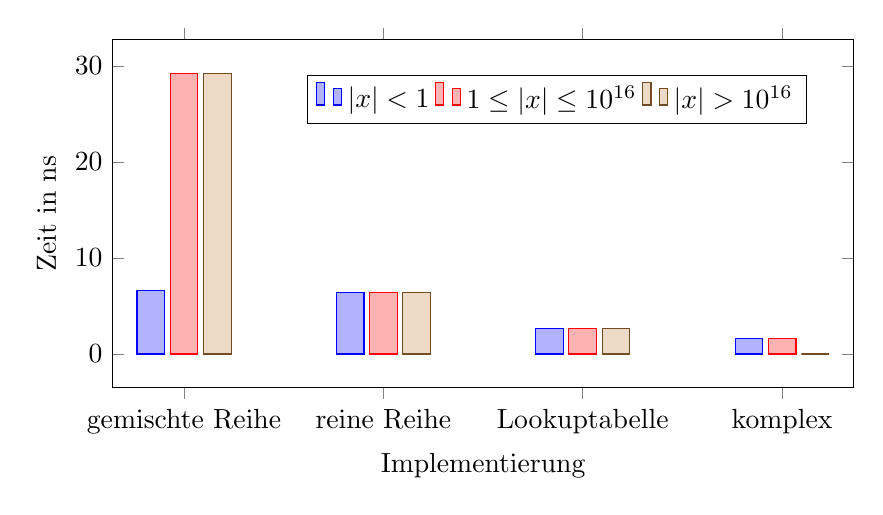
\begin{tikzpicture}
         \begin{axis}[
             width = 11 cm,
             height = 6 cm,
             ybar,
             enlargelimits = 0.12,
             symbolic x coords = {gemischte Reihe, reine Reihe,  Lookuptabelle,  komplex},
             xtick={gemischte Reihe, reine Reihe, Lookuptabelle, komplex},
             ylabel={Zeit in ns},
             xlabel={Implementierung},
             legend style={at={(0.6, 0.9)},
               anchor=north,legend columns=-1},
                            ]

             \addplot coordinates {(gemischte Reihe, 6.569) (reine Reihe,6.369) (Lookuptabelle, 2.613) (komplex, 1.648)};
             \addplot coordinates {(gemischte Reihe, 29.212) (reine Reihe, 6.369) (Lookuptabelle, 2.613) (komplex, 1.648)};
             \addplot coordinates {(gemischte Reihe, 29.212) (reine Reihe,6.369) (Lookuptabelle, 2.613) (komplex, 0.0)};
             \legend{$|x|<1$, $1\leq |x| \leq 10^{16}$, $|x|>10^{16}$};
         \end{axis}
     \end{tikzpicture}
 
     \subsection{Bewertung, Einordnung und Erklärung der Ergebnisse}
     %Folgerungen

     Wie in der Abbildung zu sehen gibt es starke Performanzunterschiede zwischen den verschiedenen Implementierungen. Wir betrachten zunächst die Implementierung mit komplexen Instruktionen. Wie zuvor erwähnt, arbeiten Funktionen der C-Mathematikbibliothek mit Hardwareoptimierungen. Damit ist die Funktion im Vergleich zu den anderen Implementierungen deutlich schneller. Es offenbart sich hierbei auch innerhalb der Funktion eine signifikante Diskrepanz zwischen den Eingabewerten unterhalb von $10^{16}$ und jenen oberhalb von $10^{16}$. 
     Ab dem gewählten Grenzwert von $10^{16}$ wird die Näherung $arsinh(x) = ln(2x)$ für die Berechnung verwendet. Diese Berechnung wird bei Optimierungsstufe O3 so stark optimiert, dass sogar bei $10^{12}$ Iterationen des Funktionsausfrufs eine kaum noch messbare Laufzeit zustande kommt. Für den Großteil der Werte deren Betrag kleiner ist als $10^{16}$ sind allerdings neben der Logarithmusberechnung zudem Multiplikation, Addition und Wurzelberechnung für die exakte Berechnung erforderlich, wodurch die Funktion in diesem Intervall eine durchschnittliche Laufzeit von etwa 1.648 ns hat. 

     Die Lookuptabelle hat für alle reellen Eingabewerte etwa die gleiche Laufzeit von 2.613 ns, da die Berechnung unabhängig von der Höhe des Eingabewerts ist. Durch die effiziente Hashfunktion mittels Bitmaske, die für das Mapping der Eingabewerte auf den jeweiligen Tabellenwert verwendet wird, ist diese Implementierung nur etwa 1.5 mal so langsam wie die worst-case Laufzeit der Implementierung mit komplexen Instruktionen. Neben der Hashfunktion werden nur wenige einfache Instruktionen für die lineare Interpolation benötigt, was ebenfalls zu der hohen Performanz dieser Implementierung beiträgt.

     Im Vergleich zu der Lookuptabelle, braucht die reine Reihenentwicklung für die von uns beschlossene Anzahl berechneter Reihenglieder mit 6.369 ns etwa 2.5 mal so lange wie die Lookuptabelle. Dies ist damit zu begründen, dass die Reihenentwicklung deutlich mehr Multiplikationen und Summen über mehrere Reihenglieder verwendet, wodurch die Berechnung länger dauert.

     Die Reihendarstellung mit verschiedenen Reihen benötigt für $|x|<1$ etwa gleich viel Zeit wie die reine Reihenentwicklung, da derselbe Algorithmus wiederverwendet wird. Für die Approximation der Eingabewerte $|x|\geq1$ werden allerdings zwei verschiedene Reihen (TaylorLn und Restreihe) sowie einige komplexere Bitoperationen verwendet. Hierdurch benötigt diese Implementierung für $|x|\geq1$ rund 29.212 ns und damit etwa 12 mal so lange wie die Lookuptabelle. Um eine vergleichbare Genauigkeit mit den Eingabewerten $|x|<1$ zu erhalten, sind diese Operationen allerdings notwendig.

    \section{Zusammenfassung und Ausblick}

    \subsection{Zusammenfassung}
    Der Trade-off zwischen Performance, Genauigkeit und Speicherverbrauch ist für die beiden Implementierungen mit einem Tabellenlookup beziehungsweise einer Reihenentwicklung sehr unterschiedlich.
    Der Tabellenlookup ist schnell, benötigt allerdings mehr Speicherplatz, je genauere Werte zu erzielen sind.
    In der Tabellenlookup Implementierung mit insgesamt etwa 30000 zu speichernden Werten in einer Lookup-Tabelle, hat die Berechnung einen maximalen relativen Fehler von 0.02\%.

    Die reine Reihenentwicklung auf der anderen Seite liefert für etwa 49.4\% aller doubles im Intervall $[-1, 1]$ den exakten Funktionswert, wird aber für Eingabewerte nahe an Eins ungenau.
    Um das exakte Ergebnis für Eins zu erhalten wäre eine unvertretbar hohe Anzahl an Reihengliedern erforderlich, die zu hohen Performanz einbußen führen würden.
    Da jedoch der interessanteste Bereich über 1 hinausgeht, lässt sich schließen, dass die Nutzung einer reinen Reihe, egal ob für $|x|\geq1$ oder $|x|\leq1$ verwendet, für gegebene Problemstellung nicht geeignet ist.
    Die gemischte Reihe liefert für 99,8\% aller doubles den exakten Funktionswert.
    Auch für die 27 reihenglieder der ln-Taylorreihe und die 13 Reihenglieder der beiden anderen Reihen, benötigt die Reihenentwicklung verglichen mit dem Lookup für $|x|>1$ die bis zu 11-fache Zeit für die Berechnung.
    Andererseits benötigt diese über 600-mal weniger Speicherplatz für eine genaue Berechnung.

    \subsection{Anwendung}
    Welche Implementierung verwendet werden sollte, hängt von den Rahmenbedingungen ab.
    Der Areasinus Hyperbolicus findet in erster Linie Anwendung in verschiedensten Bereichen der Physik und Ingenierswissenschaften~\cite{????}.
    Für die Auswertung großer Messreihen eignet sich die Lookuptabelle besser, da Messungen in der echten Welt kleine Fehler aufweisen und die Lookuptabelle für viele Werte aufgrund der besseren Performanz schneller Ergebnisse liefert.
    Hat jedoch die exakte Genauigkeit der Ergebnisse eine höhere Priorität, so eignet sich die Reihenentwicklung mit einer geeigneten Menge an Reihengliedern deutlich besser.

    \subsection{Ausblick}

    In unserer Implementierung des $arsinh(x)$ haben wir uns auf eine reine Reihenentwicklung und eine einfache Lookup-Tabelle mit linearer Näherung beschränkt.
    Unter weniger strengen Rahmenbedingungen ließe sich die Implementierung allerdings sowohl in Bezug auf Laufzeit, als auch Genauigkeit noch signifikant optimieren.

    Ein möglicher weiterführender Ansatz ist die Verwendung von Splines in der Lookup-Tabelle:
    Statt der bisher linearen Näherung zwischen zwei Messpunkten wäre es möglich den $arsinh(x)$ in diesem Intervall durch eine Kurve anzunähern.
    Hierzu werden in der Regel Polynome vom Grad drei verwendet.~\cite{????}
    Dadurch verbessert sich die Genauigkeit, insbesondere für x-Werte die genau zwischen zwei Werten in der Lookup-Tabelle liegen deutlich, während sich die Laufzeit nur minimal erhöht.
    Dafür steigt allerdings der benötigte Speicherplatz, da nun für jedes Intervall ein Polynom gespeichert werden muss.

    Eine mögliche weitere Verbesserung des Lookup-Tables ist eine effizientere Verteilung der Tabellenwerte.
    Durch die lineare Interpolation entsteht eine höhere Ungenauigkeit, je stärker die Krümmung der arsinh Funktion ist.
    Wird an den besonders stark gekrümmten Stellen eine höhere Dichte an Messpunkten verwendet und eine geeignete Mappingfunktion erstellt, würde die Lookuptabelle bei der gleichen Anzahl an vorgespeicherten Werten deutlich genauere Ergebnisse liefern.

    Ein weiterer Ansatz wäre, eine Kombination aus Reihenentwicklung und Lookup-Tabelle zu verwenden:
    Wie bereits beobachtet, liefert die Berechnung mit einer Reihenentwicklung für x-Werte, die nicht nahe an Eins liegen, besonders genaue Ergebnisse.
    Für |x|<0.125 brauchen werden beispielsweise 13 Reihenglieder benötigt, für |x|>8 werden 13 Reihenglieder der Restreihe, sowie bis zu 33 Reihenglieder der Taylorreihe für ein exaktes Ergebnis benötigt.
    In diesen Intervallen bietet es sich an, eine reine Reihenentwicklung zu verwenden.
    In dem Intervall 0.125<=|x|<=8 werden allerdings mehr Reihenglieder benötigt, wodurch es zu Performanz einbußen kommt.
    Es wäre demnach sinnvoll in diesem Intervall eine Lookup-Tabelle zu verwenden.

    Da der Wertebereich in diesem Intervall kleiner ist, lassen sich in kleinen Lookuptabellen genauere Werte speichern, wodurch der maximale relative Fehler minimal gehalten wird.
    Dieser Ansatz zielt besonders auf die Genauigkeit des Ergebnisses ab.
    Durch die Verwendung einer Lookuptabelle erhöht sich die Performanz, da für die verbleibenden x-Werte weniger Reihenglieder berechnet werden müssen, um ein exaktes Ergebnis zu erhalten.

    Anzumerken ist zudem, dass sich insbesondere die Reihenentwicklung durch die Verwendung von Assemblerinstruktionen noch signifikant auf Laufzeit optimieren lässt.

    Die Wahl des Datentyps bietet eine weitere einfache Möglichkeit zur Erhöhung der potenziellen Genauigkeit oder zur Verkleinerung des Speicherverbrauchs.
    Gemäß IEEE 754 ~\cite{StandardforBinaryFloating} könnte auch die einfache oder vierfache Genauigkeit der Fließkommaarithmetik gewählt werden, wodurch sich die erreichbare Genauigkeit auf $23*\log10(2) \approx 6,92$ dezimale Nachkommastellen bzw. $112*\log10(2) \approx 33,72$ dezimale Nachkommastellen respektive verändern würde.
    Der Speicherverbrauch würde sich respektive halbieren oder verdoppeln.

    % TODO: Fuegen Sie Ihre Quellen der Datei Ausarbeitung.bib hinzu
    % Referenzieren Sie diese dann mit \cite{}.
    % Beispiel: CR2 ist ein Register der x86-Architektur~\cite{intel2017man}.
    \bibliographystyle{plain}
    \bibliography{Ausarbeitung}
    % Sämtliche in der Ausarbeitung verwendeten Quellen sind hier aufzuführen.
    % Es sollen nur zitierfähige Quellen verwendet werden. Wir empfehlen die Verwendung von BibTEX.

\end{document}